\chapter{Origins of language strategies}
\label{s:composition}
\is{language strategy!origins of}

In \partref{s:language-strats}, I have explored the semantic and
syntactic templates behind some of the language strategies for
colour. In this chapter I will explore the origins of these
templates. The semantic templates are considered to be the result of a
combinatorial search process of basic cognitive operators. On the
syntactic side, the templates are implicitly represented in repair
strategies which can be used to express these newly generated semantic
templates. These repair strategies have been implemented and tested in
an experiment.

\section{Generation of semantic templates}
\is{semantic template!generation}

In \partref{s:language-strats}, the semantic templates were
predefined. These templates can also be generated based on a
combinatorial search process in which the cognitive primitives are
combined to form a semantic constraint network. When such a network
turns out to be successful, it can be stored by the agent and act as
a semantic template.

An illustration of such a combinatorial search process is shown in
\figref{f:composition-colour}. This search process is based on
four primitives: \textsc{Equal-to-Context}, \textsc{Filter-by-Colour},
\textsc{Filter-by-Membership} and \textsc{Select-Most-Acti\-vated}
which have been introduced in \partref{s:language-strats}. Initially
(node 1), the constraint network is empty and contains only an open
variable for the topic entity which is of type colour-entity. Next,
the search process traverses the library of primitives to find a
primitive of which the first variable is compatible to the open
variable. In this example, the library contains only one such
primitive (\textsc{Select-Most-Activated}). The network is extended
with this primitive by making its first argument equal to the open
variable. The open variable is now removed from the list of open
variables. All but the first argument of the primitive are added to
the list of open variables. The network is evaluated, but returns no
evaluation results (node 2). The second node does have an open
variable (for the second argument of \textsc{Select-Most-Activated}),
so the search process can continue. This time the library is traversed
to find a primitive that has a first argument of type
entity-set. Three such primitives seem to be found:
\textsc{Equal-to-Context} (node 3), \textsc{Filter-by-Colour} (node~4)
and \textsc{Filter-by-Membership} (node 5). Node 3 can be evaluated,
but does not return any satisfactory results. Moreover this node also does not
have any open variables any more, so this branch can not be expanded
any further. Nodes 4 and 5 also do not return the right binding, but as
they still have open variables they can still be further explored.

\begin{figure}[htbp]
  \begin{center}
    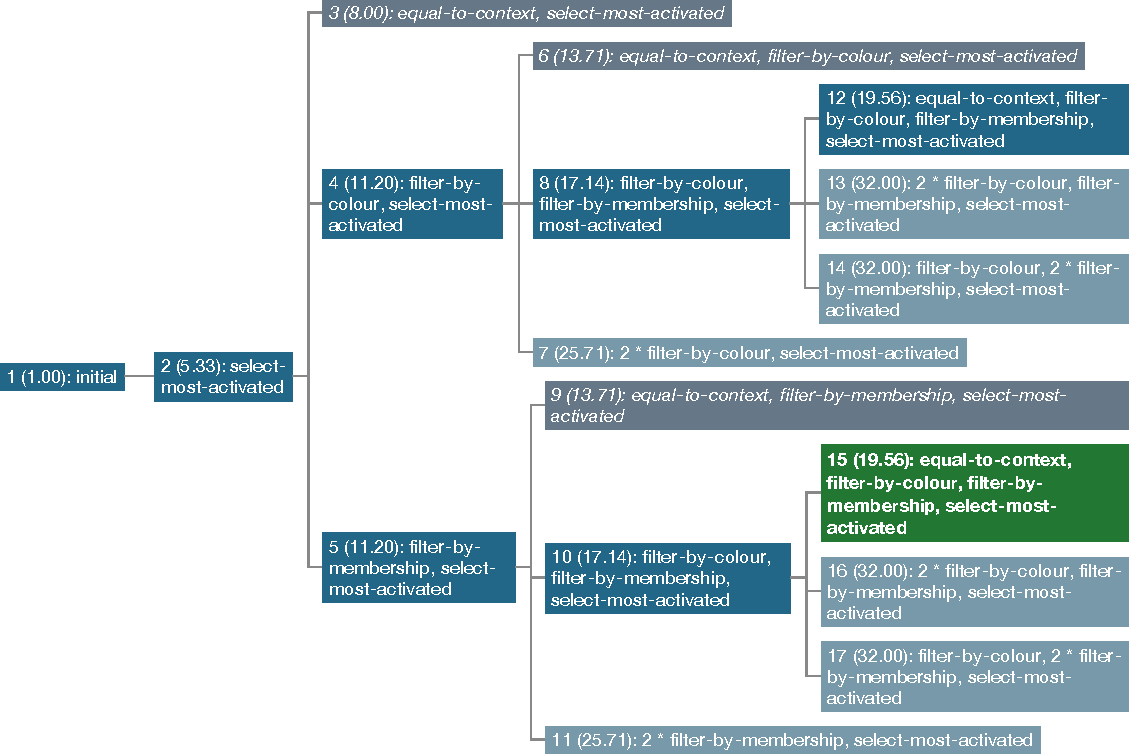
\includegraphics[width=\textwidth]{./composition/figures/composition-colour.pdf}
    \caption[Example of a combinatorial search process to construct a
    new semantic template]{Example of a combinatorial search process
      to construct a new semantic template. Each node represents one
      step in the search process in which additional primitives are
      added to the network that is being built up. When more than one
      expansion is possible the search tree splits. The green node
      (number 15) contains the solution of the current communicative
      problem. Grey nodes (for example 3 and 6) show nodes that have
      been evaluated but didn't return the correct binding for the
      topic variable. These nodes could also not be expanded any
      further. Light blue nodes (for example 7 and 11) are nodes that
      could still be explored. Blue nodes (like 4 or 5) have been
      evaluated but did not return any evaluation results.}
    \label{f:composition-colour}
  \end{center}
\end{figure}

The search process continues and finds some other interesting
networks, such as node 6, in which the network involves a single
categorisation process based on colour. This network however seems to
be insufficient to reach the current communicative goal. Finally, the
search process finds a solution for the current goal in node 15. This
network consists of two categorisation processes: one based on colour
and another based on membership. The resulting semantic network is
shown in \figref{f:composed-network}.

\begin{figure}[htbp]
  \begin{center}
    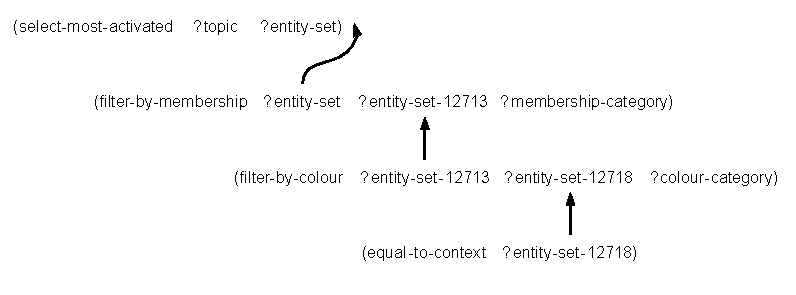
\includegraphics[width=\textwidth]{./composition/figures/composed-network.pdf}
    \caption[Example of a semantic template generated by the
    combinatorial search process]{Example of a semantic template
      generated by the combinatorial search process. It involves two
      categorisation processes. The first is based on colour and the
      second is based on membership.}
    \label{f:composed-network}
  \end{center}
\end{figure}

In order to generate the most complicated semantic templates of \partref{s:language-strats}, the search process outlined above needs to be
extended. Additional variable equalities are required that do not
involve the first argument of a primitive, like for example between
the category used in the first categorisation process and the
transformation operation of the category sets in for example the
category combination strategy. In order to account for these
networks, I have introduced another expansion operator which makes two
open variables of compatible type equal.

\section{Repair strategies}
\label{s:repair-strategies}
\is{repair strategies}

In this section I will introduce the repair strategies that allow an
agent to learn the constructions that are needed to express semantic
templates in language. Currently the main approach adopted to express
semantic constraint networks in language is identical to the one
introduced in \chapref{s:basic-strategy}. The semantic network is
divided in three layers of units: (a) entity units containing the
semantic entities, (b) functional units which make direct use of such
a semantic entity and (c) contextual units which contain any remaining
operations of the semantic constraint network that do not make direct
use of any semantic entity. This division is illustrated in \figref{f:map-structure-2} for the semantic networks shown in \figref{f:map-network-2}.

\begin{figure}
\centering
\subfigure[]{
  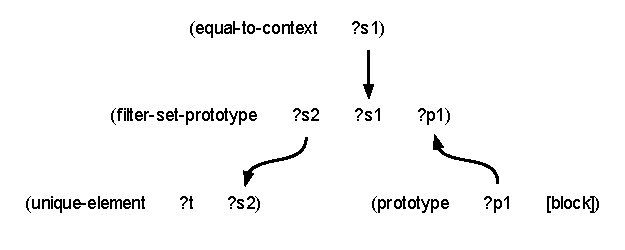
\includegraphics[width=.65\textwidth]{./composition/figures/map-network-1.pdf}
  \label{f:map-network-1}
}
\subfigure[]{
  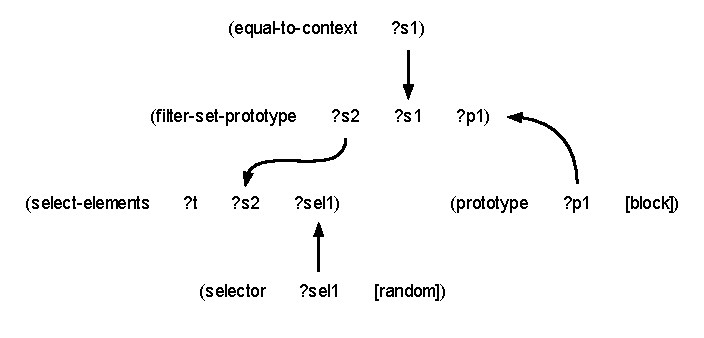
\includegraphics[width=.70\textwidth]{./composition/figures/map-network-2.pdf}
  \label{f:map-network-2}
}
\subfigure[]{
  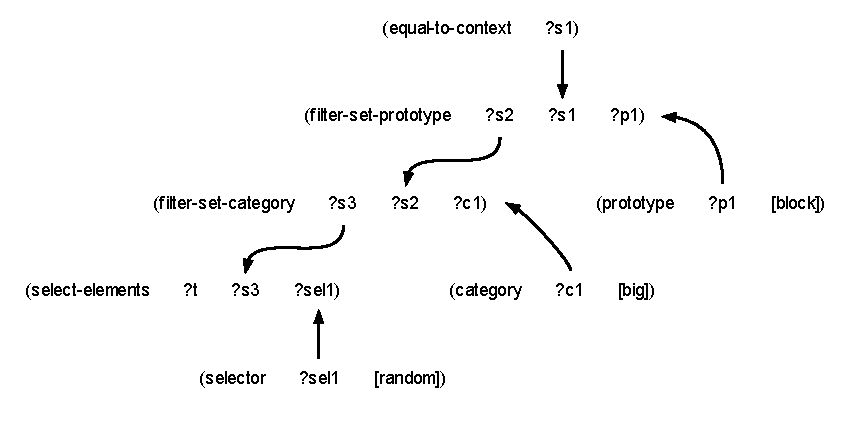
\includegraphics[width=.85\textwidth]{./composition/figures/map-network-3.pdf}
  \label{f:map-network-3}
}
\caption[Three example semantic constraint networks]{Three example semantic
  constraint networks. \subref{f:map-network-1} is the most basic network
  \subref{f:map-network-2} is a similar network in which the
  selection process is now based on random selection
  \subref{f:map-network-3} is a further extension of this network by
  adding another categorisation process between the first
  categorisation process and the selection process.}
\label{f:map-networks}
\end{figure}

\begin{figure}[htbp]
  \begin{center}
    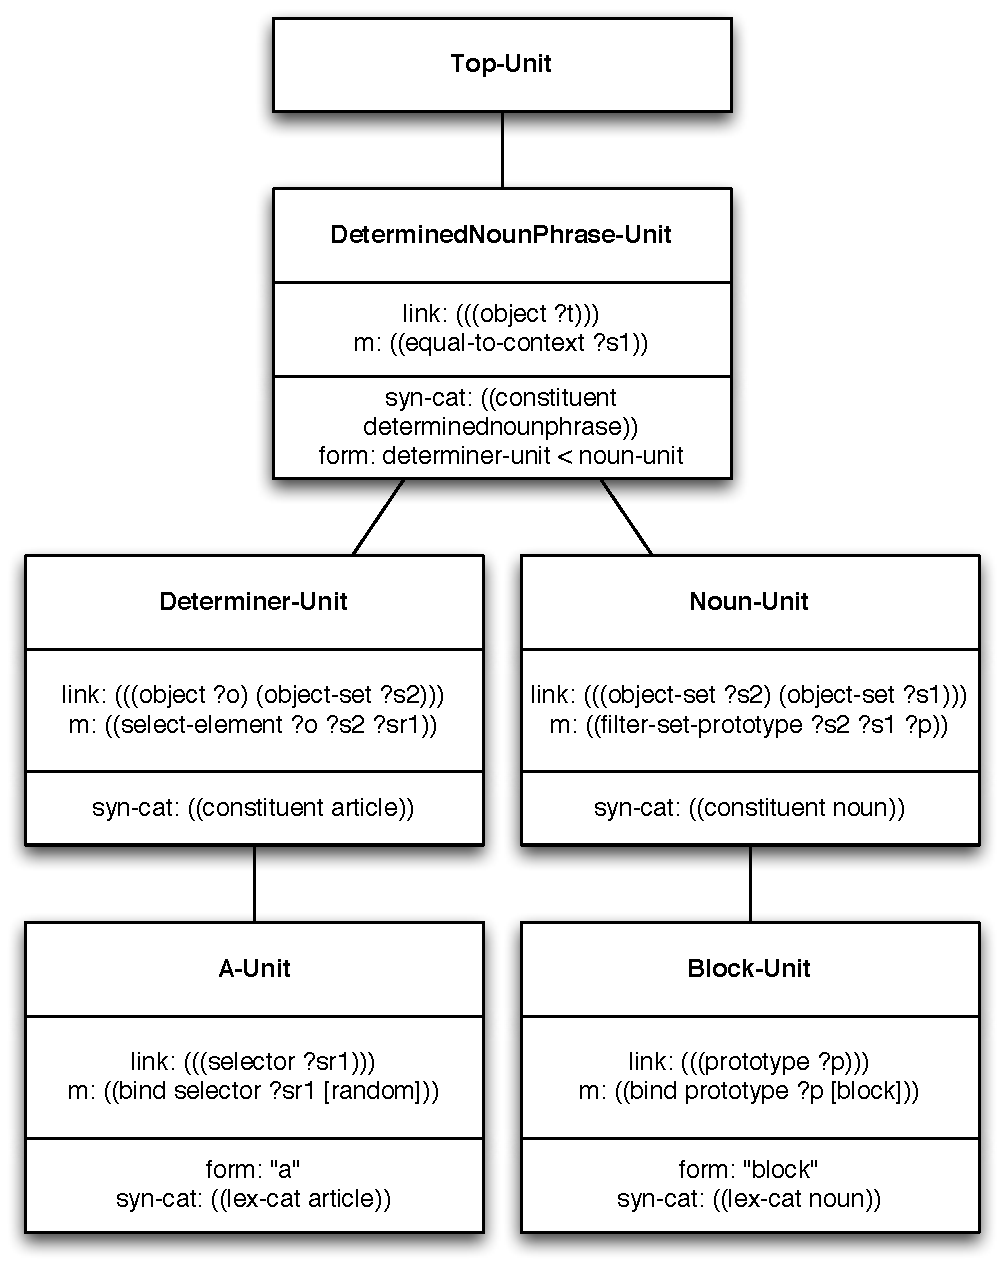
\includegraphics[width=.8\textwidth]{./composition/figures/learning-2.pdf}
    \caption[Second linguistic structure to express semantic
    constraint networks]{Linguistic structure to express the semantic
      constraint network shown in \figref{f:map-network-2},
      divided over three layers of units: entity units (Block-Unit and
      A-Unit) for the semantic entities, functional units
      (Determiner-Unit and Noun-Unit) for the primitives that directly
      use these entities and a contextual unit
      (DeterminedNounPhrase-Unit) that encapsulates all other
      primitives. Both syntactic and semantic features are shown in
      the same structure.}
    \label{f:map-structure-2}
  \end{center}
\end{figure}

\subsection{Construction of a syntactic category system}
\label{s:construction-syntactic-category-system}

The construction of the system of syntactic categories is organized as
follows: the repair strategies try to re-use any syntactic category
which would allow the re-use of a previously learned rule. If no such
syntactic category is found, the repair strategy constructs a new
syntactic category. This basic mechanism results in a one-on-one
mapping between syntactic and semantic categories at the lexical
level, but at all other levels syntactic categories are only invented
when needed and one cannot easily reconstruct a similar mapping unless
one takes into account the linguistic development of each agent.

\subsubsection{Starting from scratch}

The first time an agent has to express/interpret a semantic network
(similar to the one shown in \figref{f:map-network-1}), which
could represent the semantics of a sentence like \textit{block}) it has no
syntactic categories and hence it needs to invent two new syntactic
categories. One specifies the syntactic association between the entity
unit and the functional unit (e.g. Noun), and the other one specifies
the association between the functional unit and the contextual unit
(e.g. Noun-constituent). This kind of process is schematically shown
on the left hand side of \figref{f:map-syntactic-categories-1}.

\begin{figure}[htbp]
  \begin{center}
    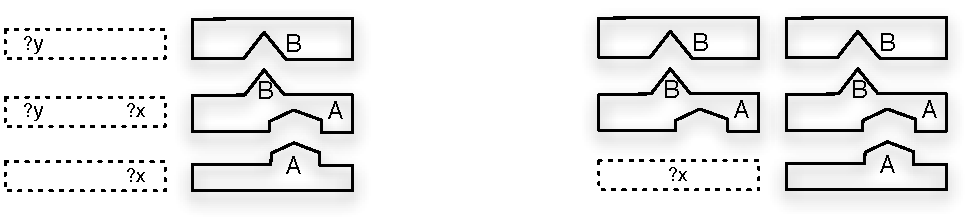
\includegraphics[width=\textwidth]{./composition/figures/mapping-1.pdf}
    \caption[First set of categories in the syntactic category
    system]{First set of categories in the syntactic category system. On
      the left: invention of new syntactic categories A, B and C. On
      the right: re-use of a syntactic category (A) as expected by the
      rule (B $\rightarrow$ A).}
    \label{f:map-syntactic-categories-1}
  \end{center}
\end{figure}

Let's suppose the agent now has to express/interpret a variation of
this semantic constraint network in which the semantic entity is a
prototype of a pyramid instead of one of a block. This provides a
first opportunity for the agents to re-use a syntactic category because
if the syntactic category of the entity unit for the pyramid would be
identical to the one of the entity unit of the block (e.g. Noun), it
would allow re-use of all the other syntactic categories (and rules) it
constructed for the previous semantic constraint network. This process
is schematised on the right hand side of \figref{f:map-syntactic-categories-1} and typically occurs at the level
of syntactic categories linking entity units and functional units.

\subsubsection{Substituting a primitive constraint}

Let us now consider a semantic constraint network in which a primitive
constraint that does not take a semantic entity as direct argument
(e.g. \textsc{Unique-Element}) is substituted by one that does so
(e.g. \textsc{Select-Ele\-ments}) (an example of such a network is shown
in \figref{f:map-network-2}). Let's suppose this network
corresponds to the semantics of a sentence like \textit{a block}. The
contextual rule of the previous example is now useless as it contains
a primitive constraint, namely \textsc{Unique-Element}, that is not
even part of the semantic constraint network at hand. The agents have
to invent a new contextual rule, but not all hope is lost, because
they can re-use every other previously introduced category (and rule)
if they incorporate the syntactic category they previously used to
associate the functional unit with the contextual unit (e.g Noun-
constituent). This process is shown in \figref{f:map-syntactic-categories-2}, and typically occurs at the level
of syntactic categories linking functional units and contextual units.

\begin{figure}[htbp]
  \begin{center}
    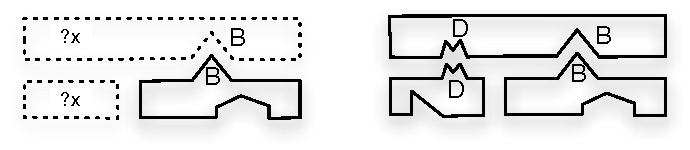
\includegraphics[width=.7\textwidth]{./composition/figures/mapping-2.pdf}
    \caption[Second set of categories in the syntactic category
    system]{Second set of categories in the syntactic category
      system. Invention of a new syntactic category (D) while reusing
      a previously learned syntactic category (B).}
    \label{f:map-syntactic-categories-2}
  \end{center}
\end{figure}

\subsubsection{Adding a primitive constraint}

The final semantic constraint network we have to consider is achieved by starting from the previous one and adding an extra
primitive constraint, \textsc{Filter-Set-Category}, in between two
existing ones, namely \textsc{Filter-Set-Prototype} and
\textsc{Select-Elements}, which could represent the semantics of a
sentence like \textit{a big block}. An example of such a network is shown
in \figref{f:map-network-3}. Using the same repair strategy as
used in the previous section, the agents could learn a new contextual
rule which combines three subunits into one new unit as shown in the
middle of \figref{f:map-syntactic-categories-3}.

\begin{figure}[htbp]
  \begin{center}
    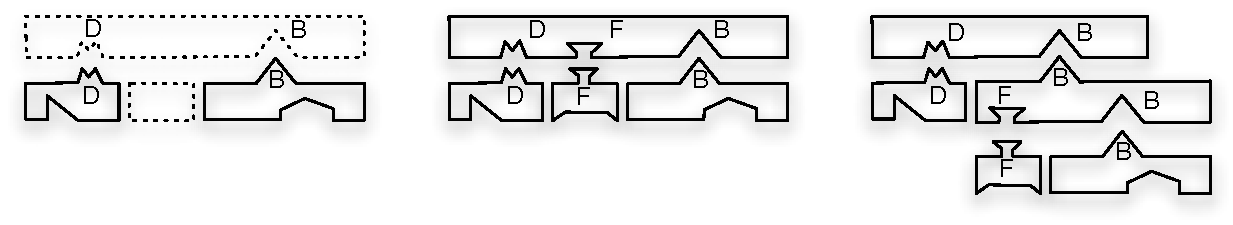
\includegraphics[width=\textwidth]{./composition/figures/mapping-3.pdf}
    \caption[Third set of categories in the syntactic category
    system]{Third set of categories in the syntactic category system. To
      the left and middle: re-use of two previously known syntactic
      categories (B and D) and invention of a new one (F) in a similar
      fashion as in the previous section. To the right: another
      solution which additionally is capable of reusing the contextual
      rule introduced in the previous section 4.2 by adding a truly
      recursive rule (B → FB).}
    \label{f:map-syntactic-categories-3}
  \end{center}
\end{figure}

But an agent can do better by exploiting another repair strategy
which allows agents to combine any number of units into one unit. In
the example shown on the right of \figref{f:map-syntactic-categories-3}, the agents are able to come up
with a rule that allows them to re-use the contextual rule introduced
in the previous section. This particular rule combines two units, one
belonging to syntactic category F (e.g. Adjective-constituent) and the
other to B (e.g. Noun-constituent). The syntactic category to which
this new combination unit should belong, determined by the deduction
mechanism introduced at the beginning of the current section, is
syntactic category B (e.g. Noun-constituent), as any other category
would block the re-use of the contextual rule. As this syntactic
category is equal to one of the rule's constituents, this new rule is
truly recursive.

This recursion becomes clear when considering a semantic network in
which another \textsc{Filter-Set-Category} is added. To express this
network no additional construction needs to be added to the rule-set of
the agent. The rules introduced above are sufficient to allow for a
complete processing of the semantic network.

\subsection{Implementaton of repair strategies}
\label{s:irl-fcg-repair-strategies}

I have implemented repair strategies allowing both speaker and hearer to
learn the grammatical rules. I will now discuss each step in more
detail. The first three repair strategies (1.1 to 1.3) take care of
learning the rules that ensure the default division in three layers of
units: (a) entity units containing the semantic entities, (b)
functional units which contain primitives that make direct use of such
a semantic entity and (c) contextual units which contain any other
primitives that do not make direct use of semantic entities.

Repair strategy 2.1, tries to optimise this process by trying to invent rules
that re-use as many previously learned rules as possible. As described
in \sectref{s:construction-syntactic-category-system}, any of
these repair strategies tries to re-use the syntactic category system
that has been built up so far as much as possible.

Let's start again with the semantic network shown in \figref{f:map-network-1}. Following the general division in three layers
of units, the target linguistic structure is shown in \figref{f:map-structure-1}. Each unit is introduced by another rule. The
repair strategies that create these rules are described below.

\begin{figure}[htbp]
  \begin{center}
    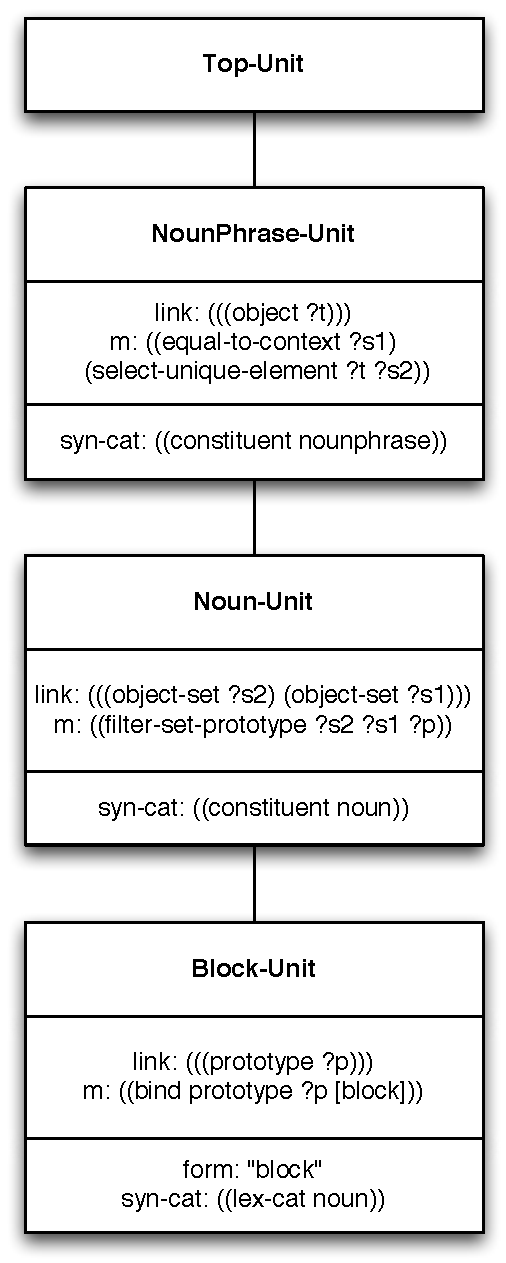
\includegraphics[width=.4\textwidth]{./composition/figures/learning-1.pdf}
    \caption[First target linguistic structure to express semantic
    constraint network]{Target linguistic structure to express the semantic
      network shown in \figref{f:map-network-1}, divided over
      three units: an entity unit (Block-Unit) for the semantic
      entity, a functional unit (Noun-Unit) for the primitive that
      directly uses that entity and a contextual unit
      (NounPhrase-Unit) that encapsulates all other primitives. Both
      syntactic and semantic features are shown in the same
      structure.}
    \label{f:map-structure-1}
  \end{center}
\end{figure}

\subsection{Repair strategy 1.1: Semantic entities}
\is{repair strategy!for semantic entities}

The diagnostic that is used to trigger this repair strategy, is that a
semantic entity is left unexpressed in the case of the speaker, or
when a unknown string is encountered by the hearer. The repair
strategy computes the required information that is used to instantiate
the template. An example of a resulting rule is shown below.

\footnotesize
\ltitle{Lexical rule for a block}
\begin{lstlisting}
((?top-unit
  (tag ?meaning 
       (meaning (== (bind prototype ?x [block])))))
 ((J ?block-unit ?top-unit)
  (link (((prototype ?x))))
  ?meaning))
<-->
((?top-unit
  (tag ?form 
       (form (== (string ?block-unit "block")))))
 ((J ?block-unit ?top-unit) 
  (syn-cat (==1 (lex-cat noun)))
  ?form))
\end{lstlisting}
\normalsize

First, the repair strategy determines which semantic entity needs to
be filled in in the meaning feature. For the speaker this is
relatively easy, as it conceptualised a meaning that it wanted to
express. The hearer has to call its conceptualisation mechanism in
order to reconstruct the semantic entity that the speaker might have
introduced. The link feature of the unit that will be introduced by
this rule is easily determined as it repeats the type and the variable
of the bind statement for the semantic entity. The repair strategy
possibly copies the syntactic category of the functional rule for the
functional primitive that will use this entity. Otherwise it
introduces a new syntactic category.

\subsection{Repair strategy 1.2: Functional primitives}
\is{repair strategy!for functional primitives}

Whenever a functional primitive (a semantic primitive that directly
uses a semantic entity) is uncovered, the repair strategy for
functional primitives is triggered. It creates a functional rule that
introduces the semantic entity to the rest of the semantic network. An
example of such a rule is shown below.

\footnotesize
\ltitle{Functional rule for FILTER-SET-PROTOTYPE}
\begin{lstlisting}
 ((?top-unit
   (sem-subunits (== ?prototype-unit))
   (tag
    ?meaning
    (meaning (== (filter-set-prototype ?s1 ?s2 ?p)))))
  (?prototype-unit
   (link (((prototype ?p))))
   (meaning (== (bind prototype ?p ?val))))
  ((J ?filter-set-prototype-unit ?top-unit (?prototype-unit))
   ?meaning
   (link (((object-set ?s1) (object-set ?s2))))))
  <-->
((?top-unit 
  (syn-subunits (== ?prototype-unit)))
 (?prototype-unit 
  (syn-cat (==1 (lex-cat noun))))
 ((J ?filter-set-prototype-unit ?top-unit (?prototype-unit))
  (syn-cat (==1 (constituent noun)))))
\end{lstlisting}
\normalsize

The rule is constructed as follows. The meaning feature contains the
functional primitive that needs to be covered. For each of the
semantic entities the primitive uses, a different subunit is
created. At the semantic side the links of these units are used to
introduce variable equalities between the semantic entities and the
arguments of the functional primitive. At the syntactic side these
units are specified through the syntactic categories of these
subunits.  On the semantic side, the new unit that is introduced by
this rule will have have a link feature that contains the variables of
arguments of the functional rule that are not provided by any of the
subunits. At the syntactic side, the new unit might introduce a new
syntactic category, unless a contextual rule could be triggered that
would impose a specific syntactic category on the new unit.

\subsection{Repair strategy 1.3: Contextual primitives}
\is{repair strategy!for contextual primitives}

The primitives that do not make direct use of semantic entities are
grouped together in a \emph{contextual unit}. This unit is introduced
by the application of a \emph{contextual rule}. 

An example of such a rule for the contextual primitives of the
semantic network shown in \figref{f:map-network-1} is given
below. It encapsulates two primitives, \textsc{Equal-To-Context} and
\textsc{Select-Unique-Element}. It requires one subunit to be present
in the structure which is of syntactic category NounConstituent and
which has as link feature two object sets. In parsing, it will ensure
the variables in these links are made equal to the variables of the
semantic primitives it contains. The newly introduced unit will be of
a newly invented syntactic category, Constituent NounPhrase, and will
have as link feature the first argument of the
\textsc{Equal-To-Context} primitive.

\footnotesize
\ltitle{Contextual NounPhrase rule}
\begin{lstlisting}
((?top-unit
  (sem-subunits (== ?subunit-1))
  (tag ?meaning
       (meaning (== (equal-to-context ?s2) 
                    (select-unique-element ?o ?s1)))))
 (?subunit-1 
  (link (((object-set ?s1) (object-set ?s2)))))
 ((J ?nounphrase-unit ?top-unit (?subunit-1))
  ?meaning
  (link (((object ?o))))))
<-->
((?top-unit 
  (syn-subunits (== ?subunit-1)))
 (?subunit-1 
  (syn-cat (==1 (constituent noun))))
 ((J ?nounphrase-unit ?top-unit (?subunit-1))
  (syn-cat (==1 (constituent nounphrase)))))
\end{lstlisting}
\normalsize

The repair strategy constructs these rules as follows. The meaning
consists of all the contextual primitives. For each of the functional
primitives, a subunit is created. At the semantic side, these subunits
specify the links of the units. On the syntactic side, the syntactic
categories of the units are specified. The unit that is introduced will
have as link feature the target entity of the semantic network it
captures.

\subsection{Re-use of syntactic categories}

As outlined above, syntactic categories are re-used as much as
possible to keep the resulting grammar as small as absolutely
necessary. One suc example of re-use can be illustrated by considering
a semantic network similar to the one shown in \figref{f:map-network-1}. The only difference to this network would be
that instead of a prototype of a block, the prototype of a ball is
used.

Repair strategy 1.1 will be triggered to invent a new rule for
this new prototype. Before it introduces a new syntactic category, it
will first try to underspecify this category by specifying it as a
variable. It will then try to apply other rules it already knows,
which happen to be the ones that have been described above for
repair strategies 1.2 and 1.3. After application of these rules, the
repair strategy checks which category got bound to the variable that
it specified for the syntactic category. In this case the variable
will be bound to the lexical category Noun, as this is the category
expected by the functional rule for \textsc{Filter-Set-Prototype}. The
repair strategy will then re-use this category for the newly
invented rule for the ball prototype.

This type of re-use is used by each of the repair strategies, so
syntactic categories are also re-used at the level of functional and
contextual units. This becomes apparent when studying the second
semantic network shown in \figref{f:map-network-2}. Following the
proposed division in three layers of units, the target linguistic
structure looks like \figref{f:map-structure-2}. Repair strategy 1.1
created a new rule for the semantic entity [random] and, as there is
no lexical category it can re-use, invented a new one (for example
Article). Repair strategy 1.2 took care of the
\textsc{Select-Element} primitive by inventing a new functional rule
for it and will also introduce a new constituent category. Learning
operator 1.3 invented a new contextual rule for the contextual
primitives. It was able to re-use the Constituent Noun category as it
was already present in the functional rule for
\textsc{Filter-Set-Prototype}. The resulting ArticleNoun rule invented
by repair strategy 1.3 is shown below.

\footnotesize
\ltitle{Contextual ArticleNoun rule}
\begin{lstlisting}
  ((?top-unit
    (sem-subunits (== ?article-unit ?noun-unit))
    (tag ?meaning 
         (meaning (== (set-to-context ?s1)))))
   (?noun-unit 
    (link (((object-set ?s2) (object-set ?s1)))))
   (?article-unit 
    (link (((object ?o) (object-set ?s2)))))
   ((J ?articlenoun-unit ?top-unit (?article-unit ?noun-unit))
    ?meaning
    (link (((object o))))))
  <-->
  ((?top-unit
    (syn-subunits (== ?article-unit ?noun-unit))
    (tag ?form 
         (form (== (meets ?article-unit ?noun-unit)))))
   (?noun-unit 
    (syn-cat (==1 (constituent noun))))
   (?article-unit 
    (syn-cat (==1 (constituent article))))
   ((J ?articlenoun-unit ?top-unit (?noun-unit ?article-unit))
    ?form
    (syn-cat (==1 (constituent articlenounphrase)))))
\end{lstlisting}
\normalsize

\subsection{Repair strategy 2.1: Re-use of constructions}
\is{repair strategy!re-use of constructions}

Re-use also occurs when the agent already knows a construction which
covers part of the meaning to be conveyed. The operator that handles
re-use starts from the best matching construction and tries to detect
what prevented it from being applicable. Next, it tries to construct a
rule which removes these obstructions. This could be achieved by
adding an extra unit which combines two units into one and also by
taking care of the variable equalities between the units that are
glued together.

The link of this additional unit is calculated as
outlined above, but as the links of the units might share some
variables, they should also be excluded from the link. This rule also
contains word-order constraints, which are either invented (in case of
the speaker) or deducted from the utterance (in case of the
hearer). The syntactical category is derived from the best matching
construction. If this operator would fail, the same problem is passed
on to learning operator 1.3, which will invent a new rule for the
contextual primitives.

This repair strategy will trigger for example when the semantic
network in \figref{f:map-network-3} needs to be expressed in
language. Let's suppose repair strategy 1.1 took care of inventing a
new entity rule for the category [big] and repair strategy 1.2
invented a functional rule for the \textsc{Filter-Set-Category}
primitive. The ArticleNoun rule described above now almost
triggers and actually covers all the meaning the producing agent needs
to express. The main issue is that this rule expects two subunits
instead of three, and that the variable equalities are also wrong. Learning
operator 2.1 now invents a rule that combines two subunits into one
and also takes care of the link features. The resulting AdjectiveNoun
rule is shown below. All other rules remain as they were, but the
resulting linguistic structure shown in \figref{f:map-structure-3}
is now hierarchical.

\footnotesize
\ltitle{AdjectiveNoun rule}
\begin{lstlisting}
((?top-unit 
  (sem-subunits (== ?noun-unit ?adjective-unit)))
 (?noun-unit 
  (link (((object-set ?s2) (object-set ?s1)))))
 (?adjective-unit 
  (link (((object-set ?s3) (object-set ?s2)))))
 ((J ?adjectivenoun-unit ?top-unit (?noun-unit ?adjective-unit))
  (link (((object-set ?s3) (object-set ?s1))))))
<-->
((?top-unit
  (syn-subunits (== ?noun-unit ?adjective-unit))
  (tag ?form 
       (form (== (meets ?adjective-unit ?noun-unit)))))
 (?noun-unit
  (syn-cat (==1 (constituent noun))))
 (?adjective-unit 
  (syn-cat (==1 (constituent adjective))))
 ((J ?adjectivenoun-unit ?top-unit (?noun-unit ?adjective-unit))
  ?form
  (syn-cat (==1 (constituent noun)))))
\end{lstlisting}
\normalsize

\begin{figure}[htbp]
  \begin{center}
    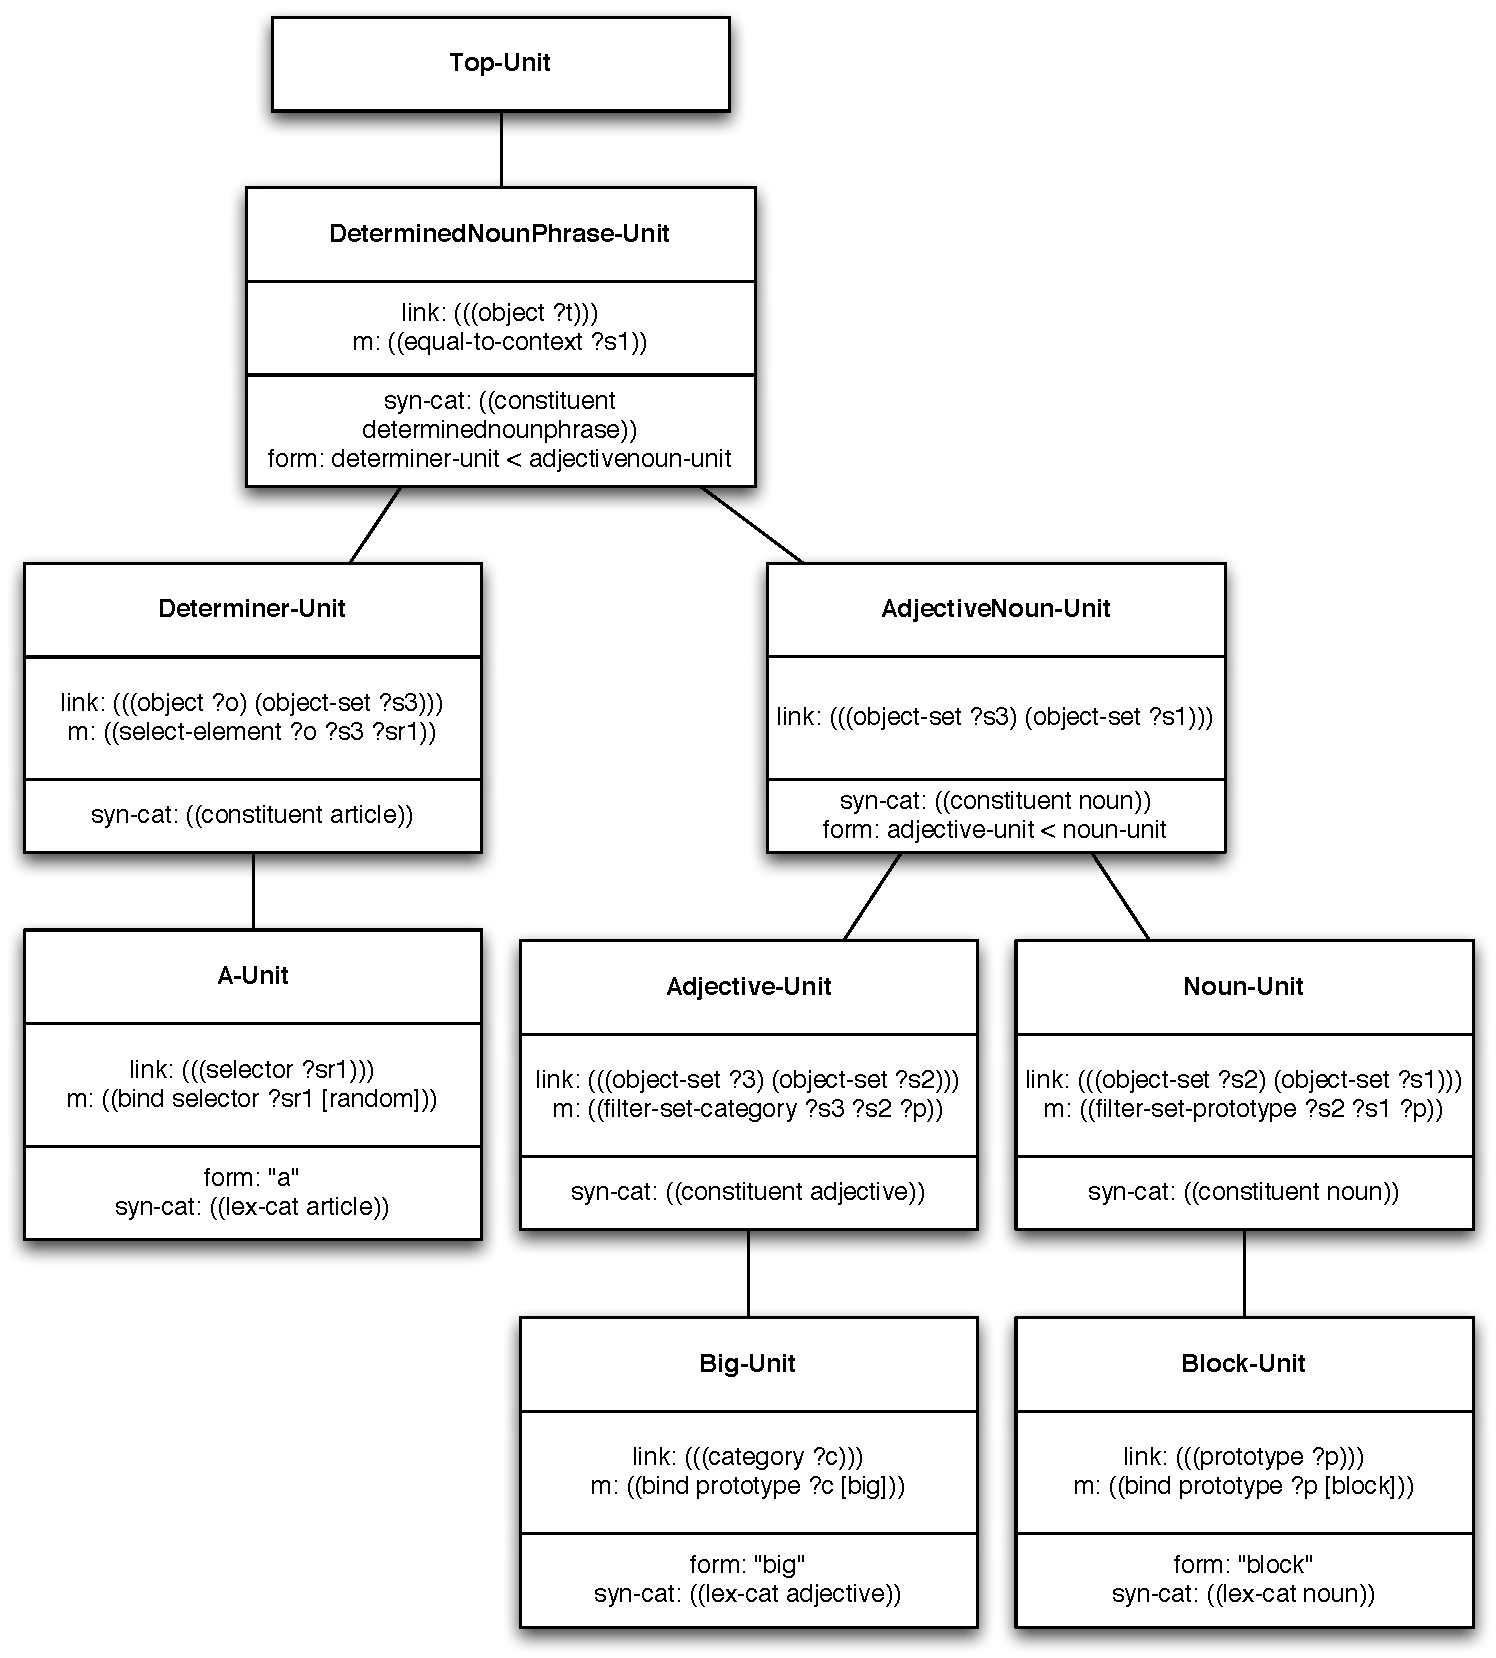
\includegraphics[width=\textwidth]{./composition/figures/learning-3.pdf}
    \caption[Third resulting linguistic structure to express semantic
    constraint networks which is hierarchical]{Resulting hierarchical structure
      to express the semantic network shown in \figref{f:map-network-2}. Repair strategy 2.1 invented an
      AdjectiveNoun rule that combines the Adjective-Unit and the
      Noun-unit into one unit by introducing the
      AdjectiveNoun-Unit. Throughout the re-use of the syntactic
      categories, this rule is also truly recursive.}
    \label{f:map-structure-3}
  \end{center}
\end{figure}

The resulting rule is recursive due to the re-use principle of
syntactic categories. The syntactic categories of the subunits are
the constituents of the functional rules for the
\textsc{Filter-Set-Category} and the \textsc{Filter-Set-Prototype}
primitive. The syntactic category of the unit it introduces during
application is imposed by the ArticleNoun rule. This category is equal
to the subunit for the \textsc{Filter-Set-Prototype} (in this case
Constituent Noun). As one of the syntactic categories of the subunit
is equal to the syntactic category of the new unit, this rule is truly
recursive.

\subsection{Experimental results}
\label{s:irl-fcg-experimental-results}

The repair strategies discussed in \sectref{s:irl-fcg-repair-strategies} have been implemented and explored
in multi-agent simulations. This experiment is scaffolded in the sense
that the world and the conceptualisation component are bypassed. This
way, I am able to focus on the development of the repair strategies in
an ideal setting.

In the experiment, the complexity of the semantic networks offered to
the language component is controlled by the experimenter and is
divided into learning stages. Each learning stage extends the previous
learning stage by a new challenging constraint network. The first four
learning stages are similar to the different examples discussed
before. The fifth one incorporates a different filtering operation
which modifies the category it uses (similar to an Adverb as in \textit{a
very big ball}) and the sixth one extends this by another filtering
operation. The next stage introduces another primitive constraint
which constrains objects based on a relation between them (like for
instance \textit{a ball in a box}). The final learning stage extends this
by incorporating another filtering operation.

The graph depicting the dynamics of the experiment is shown in \figref{f:map-repair-strategies-graph}. The size of the population is
10. Each time the learning stage is increased, the language of the
agents experiences a period of turbulence after which the communicative
success of the agents stabilises on perfect communicative success. At
each stage in which new semantic entities are used by the semantic
constraint networks, the lexicon sizes of the agents overshoot before
settling down on a one-on-one mapping between semantic entities and
lexical entries. On the level of grammatical rules one can observe a
similar pattern but this should be interpreted as the agents trying to
reach a consensus on which word-order they will use to express a
certain combination of syntactic categories (for example putting the
Article before or after the Noun). One can also observe the agents are
not inventing new grammatical rules for each level of complexity which
points to the fact that the agents are truly re-using their
grammatical knowledge.

\begin{figure}
  \begin{center}
    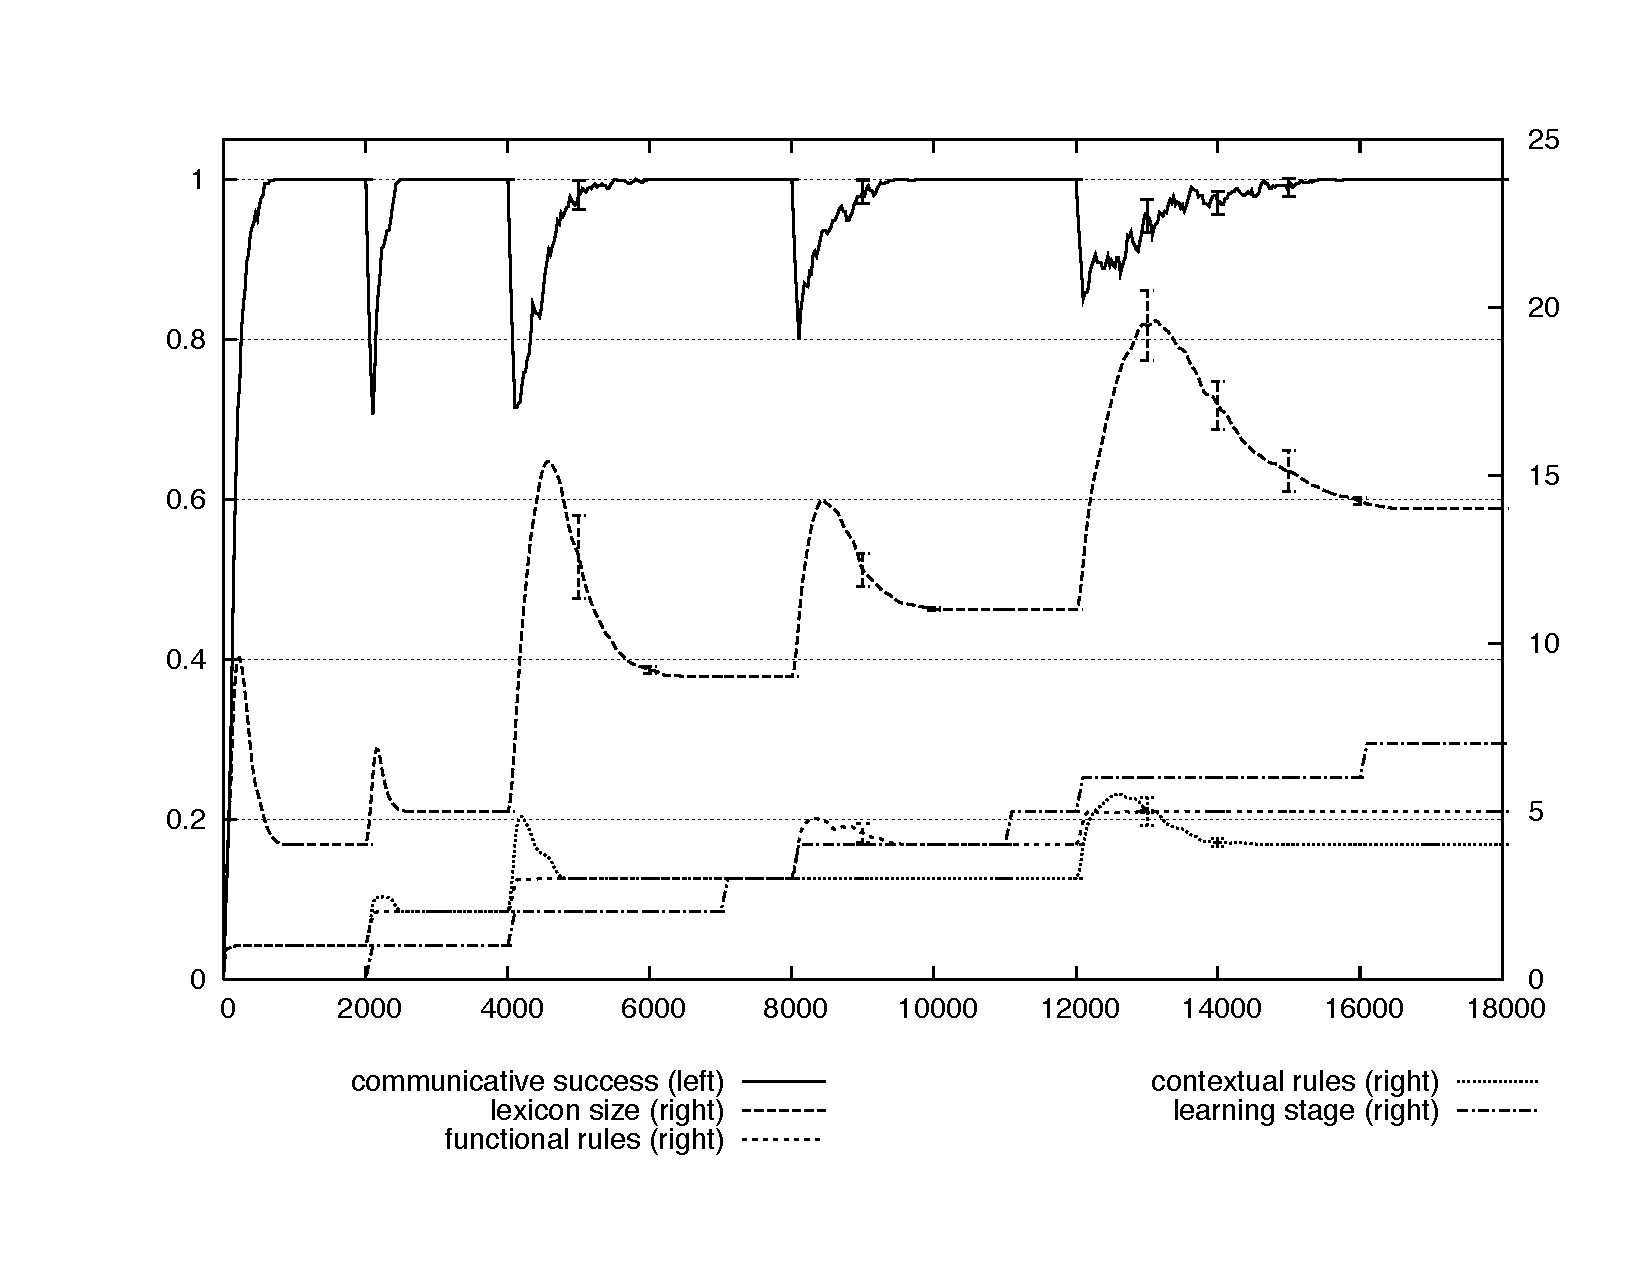
\includegraphics[width=.8\textwidth]{./composition/figures/learning-operators-graph.pdf}
    \caption[Resulting dynamics of repair strategies for predefined
    conceptualisations]{Dynamics of a multi-agent simulation in which
      the agents deploy the repair strategies introduced in \sectref{s:irl-fcg-repair-strategies}. The semantic networks they
      need to express increase in complexity over time (as shown by
      the learning stage). At each increase of the learning stage, the
      communicative success of the agents drops because they have to
      align new constructions. Once the agents have aligned their
      constructions, the communicative success becomes maximal again.}
    \label{f:map-repair-strategies-graph}
  \end{center}
\end{figure}

\section{Conclusion}

In this chapter I have introduced the general combinatorial search
process that can construct semantic templates and repair strategies to
express semantic templates in a compositional manner. These strategies
try to maximise the re-use of previously learnt grammatical rules and
to construct a system of syntactic categories that is as economical as
possible. These principles lead to interesting phenomena, such as the
emergence of recursive grammatical rules. The resulting rules are
compositional, which allow the agents to express more complex meaning
without inventing additional linguistic rules.

\newpage
\thispagestyle{empty}